\section{Background}
\label{clicknp:sec:background}

\subsection{Performance Challenges of Software Virtual Networks and Network Functions}

Virtual networks are typically implemented with virtual switch software, such as Open vSwitch \cite{pfaff2015design}.
To enhance the performance of virtual networks and meet programmability requirements, cloud service providers have redesigned software virtual switches.
By leveraging high-speed network packet processing technologies such as DPDK \cite{dpdk}, and running CPU cores in polling mode, the cost of packet processing can be significantly reduced by bypassing the OS network protocol stack.
%SoftNIC \cite{han2015softnic} proposes to implement the solidified functions in the network card with software to improve flexibility.
However, even for simple network packet forwarding that does not do any processing, each CPU core can only handle 10 M to 20 M packets per second \cite{martins2014clickos,netbricks}, which still requires 3 to 6 CPU cores for a 40 Gbps line speed of 60 M packets per second.

Traditional network functions are implemented by dedicated devices deployed at specific locations in the data center, such as F5 load balancers \cite{f5-load-balancer}. These dedicated network function devices are not only expensive, but also not flexible enough to support multi-tenancy in cloud services.
To support flexible network functions, cloud service providers also deploy software-implemented virtual network functions. For instance, Ananta \cite {ananta} is a software load balancer deployed in Microsoft data centers, used to provide cloud-scale load balancing services.
To support multiple network functions on a single server, RouteBricks \cite {routebricks}, xOMB \cite{anderson2012xomb} and COMB \cite{comb} adopt the programming model of the Click modular router \cite{kohler2000click}, implementing each network function as a C++ class, allowing each packet to be processed by various network functions in sequence on a CPU core, the so-called "run-to-completion" model.
These works show that under actual network functions, the speed of packet forwarding per server based on multi-core x86 CPUs can reach 10 Gbps, and capacity can be expanded through multi-core and building more network node clusters.
To achieve isolation between network functions, NetVM \cite{hwang2015netvm}, ClickOS \cite{martins2014clickos}, HyperSwitch \cite{ram2013hyper}, mSwitch \cite{eisenbud2016maglev} and other works put each network function in a (lightweight) virtual machine, and let the virtual switch distribute packets to these virtual machines for processing in sequence, the so-called "pipeline" model.
In the pipeline model, packets are repeatedly passed between cores, which is costly.
NetBricks \cite{netbricks} returned to the "run-to-completion" model, but implemented network functions in high-level languages, and ensured isolation between network functions at the compiler and runtime framework level.
NFP \cite{sun2017nfp} improves packet processing performance by using multiple parallel network function pipelines.

Although virtual switches and network functions implemented via software can support higher performance with more CPU cores and larger network node clusters, this will significantly increase asset and operating costs \cite {ananta,duet}.
The profitability of Infrastructure as a Service (IaaS) cloud service providers is the difference between the price customers pay for virtual machines and the cost of hosting these virtual machines.
Given that the asset and operating costs of each server are essentially determined at the time of deployment, the most effective way to reduce the cost of hosting virtual machines is to package more customer virtual machines on each computing node server and decrease the number of servers for network and storage nodes.
Currently, the price of a physical CPU core (2 hyperthreads, i.e., 2 vCPUs) is approximately $0.1 per hour, meaning the maximum potential income is around $900 per year \cite{smartnic}.
In data centers, servers usually serve for 3 to 5 years, so the highest price of a physical CPU core during the server's life cycle can reach $4500 \cite{smartnic}.
Even considering that some CPU cores are always unsold, and the cloud often offers discounts to large customers, compared with dedicated hardware, even dedicating a physical CPU core to virtual networking is quite costly.

To accelerate virtual networks and network functions, previous work has proposed using GPUs \cite {packetshader}, Network Processors (NP) \cite {cavium,netronome} and hardware network switches \cite {duet}.
GPUs were initially used primarily for graphics processing, but in recent years have expanded to other applications with massive data parallelism.
PacketShader \cite {packetshader} demonstrates that using GPUs can achieve a packet switching speed of 40Gbps.
GPUs are suitable for batch operations, but batch operations can lead to high latency.
For instance, the forwarding latency reported by PacketShader \cite {packetshader} is about $200 \mu{}s$, which is two orders of magnitude higher than \name{}.
As discussed in section \ref{smartnic-fpga}, compared with GPUs, FPGAs can fully utilize pipeline parallelism, data parallelism and request parallelism to achieve low-latency, high-throughput packet processing.
Network processors are specifically used for processing network traffic and have many hard-wired network accelerators.
NP-Click \cite{shah2004np} implemented the Click programming framework on network processors.
The year after the Click modular router \cite{kohler2000click} was proposed, NP-Click \cite{shah2004np} implemented the Click programming framework on network processors.
As discussed in section \ref{smartnic-np}, the main problem with network processors is that single-flow throughput is limited by single-core performance.
As discussed in section \ref{background:sec:network-function}, the main problem with hardware network switches is insufficient flexibility and lookup table capacity \cite {duet}.

As discussed in Section \ref{smartnic-fpga}, utilizing FPGA for network function processing poses a series of challenges. This paper concentrates on harnessing massive parallelism and programming toolchains. Compared to CPUs or GPUs, FPGAs typically have lower clock frequencies and smaller memory bandwidth. For instance, the typical clock frequency of an FPGA is about 200MHz, an order of magnitude slower than a CPU (2 to 3~GHz). Similarly, the bandwidth of a single block of memory or external DRAM on an FPGA is usually 2 to 10~GBps, while the DRAM bandwidth of an Intel Xeon CPU is about 60~GBps, and the GDDR5 or HBM bandwidth of a GPU can reach hundreds of GBps. However, CPUs or GPUs only have a limited number of cores, which restricts parallelism. FPGAs have a large amount of built-in parallelism. Modern FPGAs may have millions of LEs, hundreds of K-bit registers, tens of M-bit BRAMs, and thousands of DSP modules. Theoretically, each of them can work in parallel. Therefore, thousands of parallel "\textit{cores}" may be running simultaneously inside an FPGA chip. Although the bandwidth of a single BRAM may be limited, if thousands of BRAMs are accessed in parallel, the total memory bandwidth can reach several TBps! Therefore, to achieve high performance, programmers must fully utilize this massive parallelism.

Traditionally, FPGAs are programmed using hardware description languages such as Verilog and VHDL. These languages are too low-level, difficult to learn, and complex to program. Therefore, the large software programmer community has been far from FPGAs for many years~\cite{bacon2013fpga}. To simplify FPGA programming, the industry and academia have developed many high-level synthesis tools and systems, aiming to convert programs in high-level languages (mainly C) into hardware description languages. However, as the next subsection will discuss, they are not suitable for network function processing, which is the focus of this work.

\subsection{FPGA-based Network Function Programming}

The aim of this chapter is to leverage FPGAs to construct a multi-functional, high-performance network function platform. Such a platform should meet the following requirements.

\textbf{Flexibility.} The platform should be \textit{fully programmed in high-level languages.} Developers should be able to program using high-level abstractions and familiar tools, just like programming on multi-core processors. This is a prerequisite for most software programmers to use FPGAs.

\textbf{Modularity.} The network function platform should support a \textit{modular architecture} for packet processing. Previous experiences with virtualized network functions have shown that the correct modular architecture can capture many common functions in packet processing~\cite{kohler2000click,martins2014clickos}, making them easy to reuse in various network functions.

\textbf{High performance, low latency.} Network functions in data centers should process a large number of packets at line rates of 40 / 100~Gbps, with ultra-low latency. Previous work has shown~\cite{rollback-mb} that even a few hundred microseconds of latency added by network functions can negatively impact the service experience.

\textbf{Support for CPU/FPGA joint packet processing.} FPGA is not a panacea. As discussed in Section \ref{smartnic-fpga}, not all tasks are suitable for FPGAs. Larger logic cannot be accommodated in FPGAs. Therefore, fine-grained processing separation between the CPU and FPGA should be supported. This requires high-performance communication between the CPU and FPGA.

FPGAs have long been used to implement network routers and switches. NetFPGA \cite{lockwood2007netfpga} proposed an open hardware platform for implementing routers on FPGAs. In recent years, FPGAs have also been used to accelerate network functions \cite{rubow2010chimpp,lavasani2012compiling}. As early as the second year after the Click modular router \cite{kohler2000click} programming framework was proposed, Xilinx proposed Cliff \cite{kulkarni2004mapping} for implementing Click with FPGA, requiring hardware developers to implement a Click element as a hardware module using hardware description languages. Subsequently, CUSP \cite{schelle2005cusp} and Chimpp \cite{rubow2010chimpp} proposed a series of improvements, simplifying the interconnection of hardware modules and enhancing the capabilities of software-hardware co-processing and software simulation. However, the above work programs FPGAs using Verilog, VHDL, and other hardware description languages. It is well known that hardware description languages are difficult to debug, write, and modify, posing significant challenges for software personnel to use FPGAs.

To enhance the development efficiency of Field-Programmable Gate Arrays (FPGAs), manufacturers of these devices offer high-level synthesis (HLS) tools~\cite{vivado,intel-hls} capable of compiling restricted C code into hardware modules. However, these tools merely supplement the hardware development toolchain, and programmers are still required to manually insert the hardware modules generated from C language into the hardware description language project. Manual handling is also necessary for the communication between the FPGA and the host CPU. Efficient hardware development languages such as Bluespec \cite{bluespec}, Lime \cite{auerbach2010lime}, and Chisel \cite{bachrach2012chisel} \cite{bacon2013fpga,singh2011implementing,wester2015transformation} have been proposed by the academic and industrial communities, but their use requires developers to possess substantial hardware design knowledge. Gorilla \cite{lavasani2012compiling} proposed a domain-specific high-level language for packet switching on FPGAs. While high-level synthesis tools and efficient hardware development languages can enhance the work efficiency of hardware developers, they are still insufficient for software developers to utilize FPGAs.

Click2NetFPGA~\cite {Click2NetFPGA} employs high-level synthesis tools to directly compile the C++ code of Click modular routers \cite {kohler2000click} to FPGA, thereby providing a modular architecture. However, several bottlenecks exist in the system design of Click2NetFPGA's performance (such as memory and packet I/O), and the code has not been optimized to ensure fully pipelined processing, resulting in a performance that is two orders of magnitude lower than that of this paper. Moreover, Click2NetFPGA does not support FPGA/CPU joint processing, thus it cannot update configurations or read states during data plane runtime.

In recent years, to enable software developers to use FPGA, manufacturers of these devices have proposed OpenCL-based programming toolchains~\cite{aoc,sdaccel}, offering a GPU-like programming model, as depicted in Figure \ref{intro:fig:opencl}. Software developers can offload kernels written in OpenCL language to FPGA.

\begin{figure}[htbp]
	\centering
	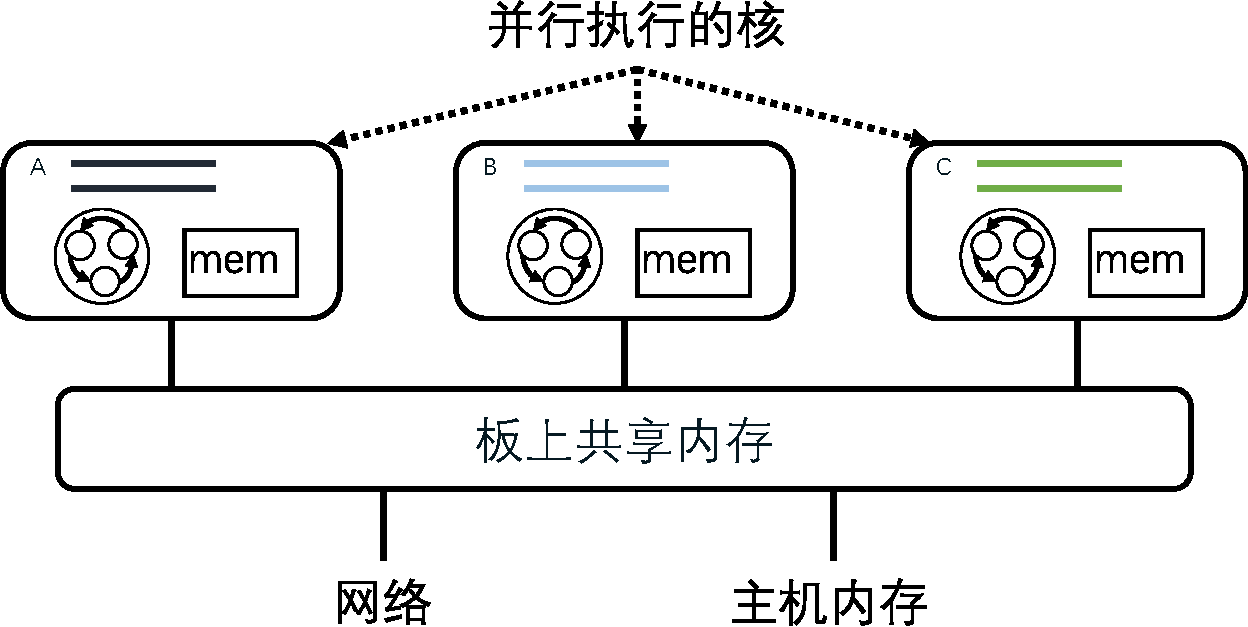
\includegraphics[width=0.7\textwidth]{../figures/opencl.pdf}
	\caption{Communication method between OpenCL kernels and between kernels and network, host: shared memory.}
	\label{intro:fig:opencl}
\end{figure}

Nonetheless, this method has its limitations. Multiple parallel executing kernels need to communicate through on-board shared memory, and the DRAM throughput and latency on the FPGA are not ideal, making shared memory a communication bottleneck. Furthermore, the communication model between FPGA and CPU resembles a GPU-like batch processing model. The communication between the host program and the FPGA kernel must always go through the on-board DDR memory. This results in higher processing latency (about 1 millisecond), which is not suitable for network packet processing that requires microsecond-level latency. Thirdly, OpenCL kernel functions require explicit calls from software programs on the host machine. Before the kernel terminates, the host program cannot control the kernel behavior, such as setting new parameters, nor can it read any kernel state. However, network functions face a continuous stream of data packets and should always be running. Lastly, OpenCL does not support joint packet processing between CPU and FPGA, and packet processing on the CPU can only be performed outside the OpenCL framework.

The following will introduce \name{}, a novel FPGA-accelerated network function platform that meets the requirements of flexibility, modularity, high performance, low latency, and CPU/FPGA joint processing.

Network packet processing belongs to stream processing. ST-Accel \cite{ruan2018st} pointed out that the efficiency of stream processing through FIFO in FPGA is higher than that of shared memory, which can achieve lower latency and higher throughput. For this reason, within the \name framework, the processing logic modules of FPGA and the communication between the network and the host should also be through the FIFO pipeline, as shown in Figure \ref{intro:fig:element_conn}.

\begin{figure}[htbp]
	\centering
	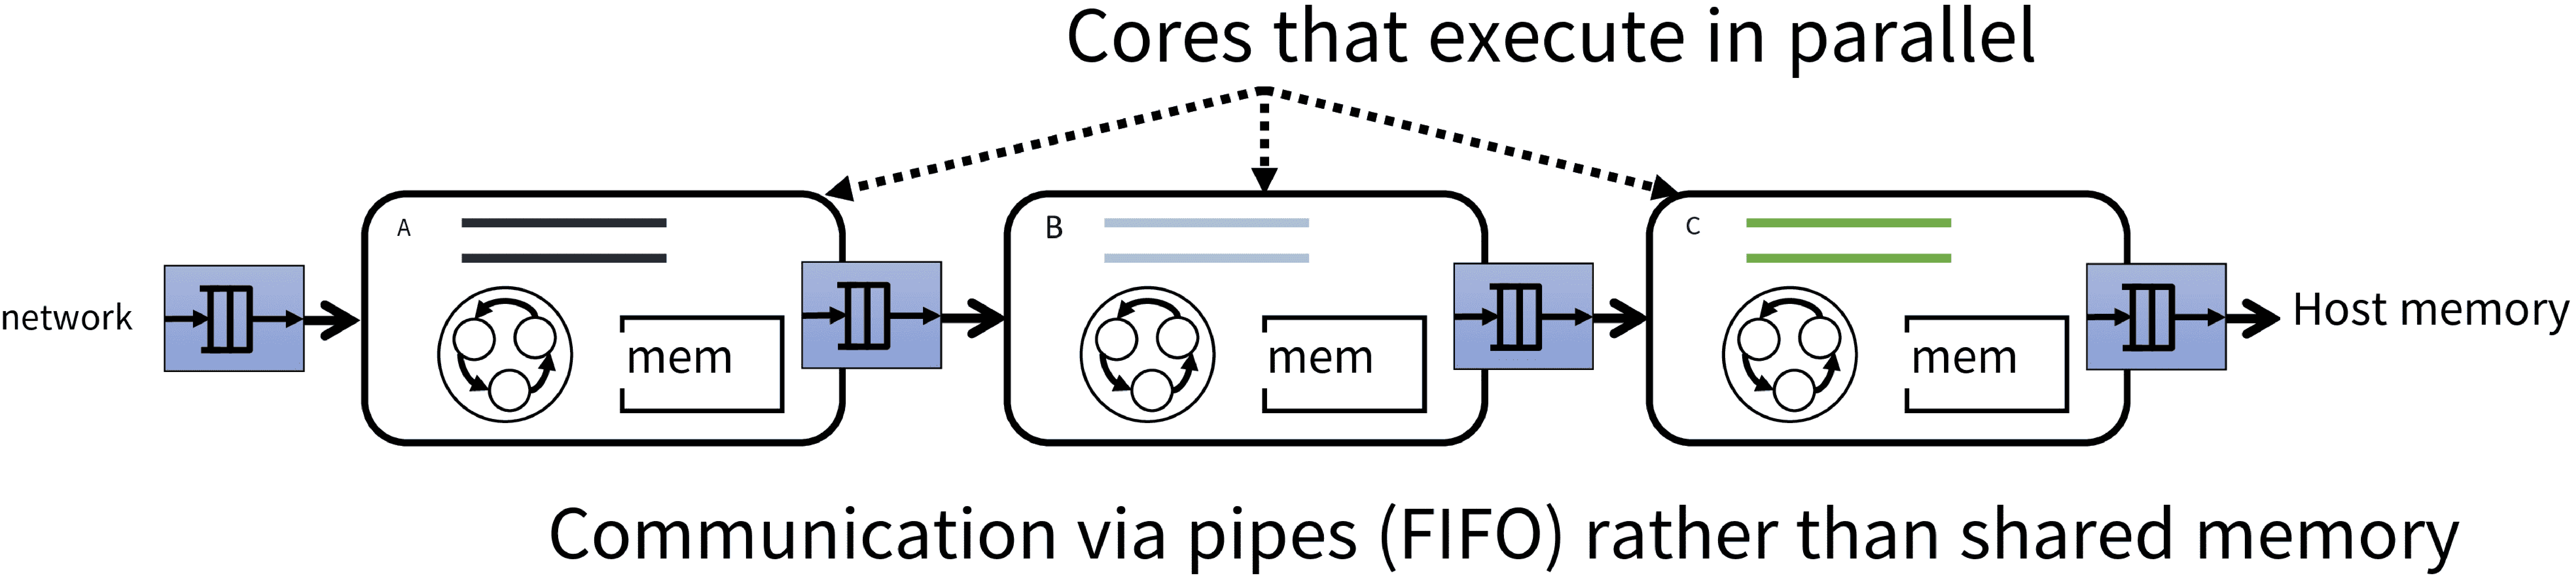
\includegraphics[width=1.0\textwidth]{image/element_conn.pdf}
	\caption{Communication method between ClickNP kernels and between kernels and network, host: pipeline (FIFO).}
	\label{intro:fig:element_conn}
\end{figure}

\egg{
Today's data centers depend on a broad array of network functions to implement network virtualization, ensure security (e.g., firewalls and intrusion detection/prevention systems), carry out measurements, and enhance performance (e.g., traffic scheduling). As data centers are transitioning towards 40 Gbps bandwidth at end hosts, where the line-rate is 60 M packets per second for minimum-sized packets, a higher throughput requirement is imposed on network processors. Moreover, as data center services are rapidly evolving, programmability becomes essential for network processors. However, existing network processors have a significant mismatch to the performance and programmability requirements.}

\subsection{Architectures for Network Processors}

Network processors based on general-purpose CPUs such as ClickOS \cite{martins2014clickos} offer excellent programmability, modularity, and composability, but the packet forwarding performance of a single core cannot keep up with a 10 Gbps line rate for minimum-sized packets, even before any network function is plugged in. Because CPU instructions are executed sequentially and have low parallelism, packet processing performance would drop further as more network functions are added. If a CPU-based network processor is added bump-in-the-wire, there will be tens of microseconds additional end-to-end latency \cite{martins2014clickos}, which is one magnitude higher than the switching fabric. In a network virtualization scenario, if packet encapsulation and decapsulation are done at end hosts, as in the case of a virtual switch, network card offloading mechanisms including Large Send Offload (LSO) and Large Receive Offload (LRO) have to be disabled, which has a significant impact on TCP performance \cite{yoshino2008performance}.

ASICs are known to be high-performance, but the network functions are fixed. Commodity switching ASICs typically have a pipeline of network functions \cite{broadcomethernet}, where each function can be configured via registers and a match table based on TCAM or memory. Some ASICs provide flexible OpenFlow-like match-action tables \cite{broadcomopenflow}, but the packet parser is fixed (we could not support new packet header and shim layer formats), actions are not extensible, and the order of network functions in the pipeline is not reconfigurable.

GPUs are extensively utilized as co-processors for tasks that require intensive computing, but their SIMD (Single-Instruction Multiple-Data) programming model is not suitable for network processing, where different packet types may follow various execution flows. The high power consumption, the high latency of batch processing, and the inability to send and receive network packets without CPU intervention also make GPU-based network processors impractical in data centers.

Fortunately, reconfigurable hardware is an architecture that offers both programmability and high performance, as well as power efficiency for certain workloads. The most notable example of reconfigurable hardware is FPGA (field programmable gate arrays). FPGAs can implement any logic function and use distributed on-chip registers and SRAM to exploit bit-level and task-level parallelism, so stream processing pipelines do not "hit the memory wall" as in Von Neumann architecture \cite{bacon2013fpga}. FPGAs have shown potential in accelerating many workloads in the cloud \cite{putnam2014reconfigurable}. Moreover, Moore's law is still applicable in the FPGA industry, as the fabrication technology of FPGA is currently several generations behind the CPU industry [citation required].

\subsection{FPGA Programming Challenge}

Despite the potential of FPGA in network processing, FPGA's programmability is traditionally provided by hardware description languages (Hardware Description Languages) such as Verilog, which require hardware knowledge and are much more difficult to program and debug than higher-level languages like C/C++. Therefore, existing FPGA-based network processors such as NetFPGA \cite{lockwood2007netfpga} are challenging to program for software engineers.

Many works, for example, OpenFlow \cite{mckeown2008openflow}, P4 \cite{bosshart2014p4}, and Software Defined Network et \cite{xilinxsdnet}, provide programmability by abstracting a set of primitives in network processing and defining a high-level programming language to compose the primitives. This approach has proven effective, but the programmability is limited to a set of predefined actions, which cannot keep up with the rapid development of data center network functions. Our work aims to make the primitives extensible for software engineers.

Fortunately, several frameworks have been proposed to provide abstractions for generic FPGA programming. Examples of such works include Xilinx Vivado High Level Synthesis \cite{feist2012vivado} based on C/C++, Altera SDK for OpenCL \cite{czajkowski2012opencl} based on C-like OpenCL and IBM Lime \cite{auerbach2010lime} based on Java.

However, FPGA has a completely different architecture than general-purpose CPUs. For software programmers that bear Von Neumann model in mind, the compilers may generate surprisingly poor hardware logic for reasonable code in high-level language. For example, Click2NetFPGA \cite{Click2NetFPGA} uses LLVM and high-level synthesis tools to compile optimized Click C++ code into hardware description language, but the resulting FPGA-based router can only process 178 K pps (packets per second) for 98B packets, and 215 Mbps for large packets, which is 30 -- 50x slower than a CPU core in ClickOS \cite{martins2014clickos}. The bottleneck for small packets is the IP header checking stage \cite{Click2NetFPGA} because this stage is not fully pipelined; the bottleneck for large packets is the byte-wide shared memory \cite{Click2NetFPGA}, indicating a shared-memory design suitable for Von Neumann model would yield poor performance on FPGA.

FPGA has millions of logic gates with 10x slower clock rate than CPU, thousands of distributed fast SRAMs each with only KB capacity, and a large DRAM with 10x lower throughput than DRAMs in CPU architecture. Consequently, exploiting both spatial and temporal parallelism is crucial to unleashing the performance of FPGA. In network stream processing, most operations are independent of each other and therefore can be either parallelized (spatial) or pipelined (temporal), so that each stage of the pipeline can process different packets in parallel.

\subsection{Design Goals}
\label{clicknp:subsec:designgoals}

We highlight several design goals for our ClickNP framework to enable software engineers to write efficient network applications.

\smalltitle{Modularity.} Modularity is one key feature that improves parallelism, since modules do not have shared state and can run in parallel by nature. Borrowing the concepts from Click modular router \cite{kohler2000click}, \textit{elements} are basic building blocks of network functions. Elements run asynchronously and are connected via uni-directional \textit{channels}. The network processing pipeline is a data flow graph of elements and channels, starting from Ethernet receivers and ending at Ethernet transmitters.

\smalltitle{Line-rate throughput.} To allow efficient processing of packet content, an Ethernet packet is split into 32-byte \textit{flits} before feeding into elements. In the worst case, when 69-byte packets are received back-to-back, the line rate would be 40G / 8 / (69+20) = 56.18 Mpps, which splits into 56.18M * 3 = 168.54M flits. Every clock cycle an element reads at most one flit and outputs zero or one flit. This means any FPGA pipeline with clock frequency lower than 168.54 MHz would not be able to achieve line rate. If we waste a cycle between every two packets, the minimum clock frequency would be 224.72 MHz. However, on Stratix V FPGA platform \cite{stratix2012device}, non-trivial hardware logic that accesses registers and local memory can hardly run higher than 200 MHz. Therefore no idle cycles are allowed in elements processing packet content. First, the framework should provide abstractions for programmers to develop fully pipelined network functions. Second, as full compilation of a FPGA program may take hours, the framework should give performance warnings in an early compilation stage if the code cannot be fully pipelined.

\smalltitle{Code reuse.} Many network applications share a common set of elements, for example packet parser, lookup tables and packet modifications. Code of these elements should be reusable and elements should be composable. Software engineers should be able to write many network applications simply by connecting elements in the library.

\smalltitle{Debugging support.} First, as hardware description language (e.g. Verilog) simulation and debugging is both time consuming and requires extensive hardware knowledge, the framework should be able to compile OpenCL-based ClickNP programs to native x86 code for emulation, and provide traffic generators and receivers to test functionality. Second, as CPU is neither capable of sending or receiving packets at 60 Mpps, we need a FPGA-based network benchmark suite to perform stress testing on the network processor.

\smalltitle{Separation of control plane and data plane.} On one hand, our throughput requirement requires most network packets to be processed through the reconfigurable hardware without any CPU intervention. On the other hand, software-defined networking and network function virtualization applications are usually complicated and have external dependencies. Therefore a clear interface between the control plane and the data plane is mandatory, where data plane programs are written within ClickNP framework and target massive parallelism, and control plane programs need only slight modifications to call our host library and perform on-the-fly reconfigurations.

\smalltitle{Host communication.} Network processors require low-latency and high-throughput interactions with the host machine. In Software Defined Networks and Network Function Virtualization applications, FPGA needs to send unknown packets to the controller and request a new forwarding rule to be inserted into FPGA. The round-trip time should be as low as possible to reduce end-to-end flow establish time. In packet replay and capture applications, FPGA needs to receive or send Gigabytes of packets from or to the host machine without using the network adapter.

We design ClickNP to meet the above design goals with Catapult FPGA \cite{putnam2014reconfigurable} and Altera OpenCL \cite{singh2011implementing}. In the next section, we will describe the FPGA and OpenCL components, and how we build a toolchain that abstracts away hardware specific details.
}

\egg{
\subsection{FPGA in datacenter}

Conventionally, datacenter operators largely relied on the performance improvements in general-purpose servers
to improve the operation efficiency. This performance improvement rate of servers 
has considerably slowed down recently due to the power limitations~\cite{putnam2014reconfigurable, more-citation}.
This has motivated the adoption of \textit{accelerator} that can be specialized to certain workloads to get efficiency gains.
However, the non-programmable ASIC-based accelerators are undesirable for datacenters due to following two reasons:
Firstly, datacenter operators prefers homogeneous server configurations to minimize the management overhead and also provide
a consistent platform that applications can rely on.
Secondly, services in datacenters evolve extremely rapidly. Waiting for the long release cycle of ASIC chips is undesirable.
%
Therefore, it requires a flexible accelerator that can potentially speed up many applications.
%
GPU and FPGA are two predominate technologies that satisfy this requirement.

% comparison between GPU and FPGA
% power efficiency
Compared with GPU, FPGA is more power efficient. For example, the latest NIVDIA xxx consumes xxx W power, while a high-end
Altera Stratix V consumes xxx W power ( J per op?) \knote{need a citation}. 
% versatile 
Further, FPGA is more versatile. While GPU is mainly designed to achieve \textit{data parallelism} with SPMD (single program, multiple data), 
FPGA can easily achieve both data parallelism and \textit{task parallelism} as different block of LEs can be independently configured to
implement different processing.  
% I/O
Finally, FPGA supports various I/O interface. Normally, GPU can only communicate with PC memory through PCIE bus. 
But FPGA can input or output data from many interfaces like network ports, and is more suitable for processing these 
I/O streams.

FPGA is a mature technology and becomes inexpensive. A large scale deployment of FPGA in Microsoft datacenter shows 
that a high-end FPGA board increases the total cost of ownership (TCO) of a server by less than 30\%, but can double 
the Bing search efficiency~\cite{putnam2014reconfigurable}.
%
In this paper, we focus on using FPGA to accelerate network functions that are essential to our datacenter networks.
}

\egg{
\smalltitle{inexpensive}

Why I need this as background:
\begin{itemize}
\item Price issue?
\item Power?
\item Transition to FPGA for network functions?
\end{itemize}
}
